\documentclass[12pt]{article}

% --- Packages ---
\usepackage{graphicx}
\usepackage{amsmath}
\usepackage{amssymb}
\usepackage[a4paper,margin=0.5in]{geometry}
\usepackage{enumitem}
\usepackage{xcolor}
\usepackage{tikz}
\usetikzlibrary{arrows.meta, shapes.geometric, decorations.pathmorphing, decorations.pathreplacing}

% --- TikZ Styles ---
\tikzstyle{element}=[draw, circle, inner sep=1pt, fill=gray!20]
\tikzstyle{phaser}=[draw, rectangle, minimum size=6pt]
\tikzstyle{divider}=[draw, circle, inner sep=0pt, minimum size=4pt]
\tikzstyle{amp}=[draw, regular polygon, regular polygon sides=3, shape border rotate=0, inner sep=0pt, minimum size=7pt]
\tikzstyle{source}=[draw, circle, minimum size=6pt, label={[label distance=-1mm]center:\tiny RF}]

% --- Fancy header/footer (fixed) ---
\usepackage{fancyhdr}
\pagestyle{fancy}
\fancyhf{} % clear all fields
\fancyhead[C]{Introduction to Radar}
\fancyfoot[L]{HW3B}
\fancyfoot[R]{Page \thepage}

\setlength{\headheight}{40pt} % satisfy fancyhdr requirement
\renewcommand{\headrulewidth}{0.4pt}
\renewcommand{\footrulewidth}{0.4pt}

% Color the rules safely
\makeatletter
\renewcommand{\headrule}{%
  {\color{red}\hrule width\headwidth height\headrulewidth}\vskip-\headrulewidth}
\renewcommand{\footrule}{%
  \vskip-\footruleskip
  {\color{red}\hrule width\headwidth height\footrulewidth}\vskip\footruleskip}
\makeatother

\begin{document}

% --- Title ---
\begin{center}
    \textbf{Introduction to Radar -- HW3B}
\end{center}

\vspace{1em}

\noindent\textbf{Reading:} POMR 2\textsuperscript{nd} ed., chapters 10, 11 and module 9.

\vspace{1em}

\noindent
Place MATLAB code at end of assignment in an appendix. You do not need to turn in the code.

\vspace{1em}

% --- Questions 1–12 ---
\begin{enumerate}[label=\arabic*., leftmargin=*, itemsep=8pt]
    \item A radar needs a power amplifier for a transmitter with the following characteristics: 50 kW peak power, 5 kW average power, 10\% bandwidth, 5 W drive power. What type of tube would be a suitable choice? Explain why.

    \vspace{0.5em}
    $\rightarrow$ A \textbf{Klystron} amplifier. It meets the high gain requirement of 40 dB ($10\log_{10}(50000/5)$), high power, and operates within the 1-10\% bandwidth range.

    \item A MESFET microwave power transistor has a phase sensitivity of 10 deg/V of bias change. The DC power supply ripple voltage is 100 mV. Calculate the spurious sideband amplitude in dBc.

    \vspace{0.5em}
    $\rightarrow \Delta\phi_{peak} = (10 \text{ deg/V})(100 \cdot 10^{-3} \text{ V}) = 1^\circ$

    \vspace{0.5em}
    $\rightarrow \Delta\phi_{rad} = 1^\circ \cdot \frac{\pi}{180^\circ} \approx 0.01745 \text{ rad}$

    \vspace{0.5em}
    $\rightarrow \text{dBc} = 20\log_{10}\left(\frac{\Delta\phi_{rad}}{2}\right) = 20\log_{10}\left(\frac{0.01745}{2}\right) = \boxed{-41.2 \text{ dBc}}$

    \item What three external subsystems does the receiver interface with?

    \vspace{0.5em}
    $\rightarrow$ The \textbf{Antenna}, the \textbf{Transmitter}, and the \textbf{Signal Processor}.

    \item What is the total noise power produced from thermal noise of a component at room temperature with 1 GHz of instantaneous bandwidth?

    \vspace{0.5em}
    $\rightarrow P_N = (-174 \text{ dBm/Hz}) + 10\log_{10}(1 \cdot 10^9 \text{ Hz}) = -174 + 90 = \boxed{-84 \text{ dBm}}$

    \item A receiver front end undergoes a two-tone test to measure IP3. The input fundamentals are located at 8.3 and 8.31 GHz. Where do the third-order intermodulation signals appear?

    \vspace{0.5em}
    $\rightarrow f_{IM3, lower} = 2f_1 - f_2 = 2(8.3 \text{ GHz}) - 8.31 \text{ GHz} = \boxed{8.29 \text{ GHz}}$

    \vspace{0.5em}
    $\rightarrow f_{IM3, upper} = 2f_2 - f_1 = 2(8.31 \text{ GHz}) - 8.3 \text{ GHz} = \boxed{8.32 \text{ GHz}}$
\end{enumerate}

\newpage

\begin{enumerate}[label=\arabic*., leftmargin=*, start=6, itemsep=8pt]
    \item Sketch diagrams of the standard phased-array feed types. For each, give one pro and one con.

    \vspace{0.5em}
    $\rightarrow$ \textbf{Constrained Series Feed:}
    \begin{center}
    \begin{tikzpicture}[scale=0.7, transform shape]
        \draw[thick] (0,0) -- (6,0) node[right, black] {Load};
        \draw[thick, <-] (0,0) -- (-1,0) node[left, black] {Input};
        \foreach \x in {1,2,3,4,5} {
            \draw (\x,0) -- (\x,0.5);
            \node[phaser] at (\x,0.75) {};
            \draw (\x,1) -- (\x,1.2);
            \node[element] at (\x,1.45) {};
            \draw[-{Stealth[length=2mm]}] (\x,1.6) -- (\x,2);
        }
    \end{tikzpicture}
    \end{center}
    \quad Pro: Simple structure. Con: Narrow bandwidth, beam squint.

    \vspace{1em}
    $\rightarrow$ \textbf{Constrained Corporate Feed:}
    \begin{center}
    \begin{tikzpicture}[scale=0.7, transform shape]
        \foreach \x in {0,1.5,3,4.5} {
             \node[element] at (\x, 2) {}; \draw[-{Stealth[length=2mm]}] (\x,2.15) -- (\x,2.5);
             \node[phaser] at (\x,1.5) {}; \draw (\x,1.75) -- (\x,1.25);
        }
        \node[divider] (d1) at (0.75, 0.75) {}; \node[divider] (d2) at (3.75, 0.75) {};
        \draw (0,1.25) -- (d1) -- (1.5,1.25); \draw (3,1.25) -- (d2) -- (4.5,1.25);
        \node[divider] (d0) at (2.25, 0) {};
        \draw (d1) -- (d0) -- (d2);
        \draw[->] (2.25, -1) node[below] {Input/Output} -- (d0);
    \end{tikzpicture}
    \end{center}
    \quad Pro: Wide bandwidth. Con: Single point of failure.

    \vspace{1em}
    $\rightarrow$ \textbf{Constrained Distributed Feed:}
    \begin{center}
    \begin{tikzpicture}[scale=0.7, transform shape]
        \foreach \x in {0,1.5,3,4.5} {
             \node[element] at (\x, 2) {}; \draw[-{Stealth[length=2mm]}] (\x,2.15) -- (\x,2.5);
             \node[phaser] at (\x,1.5) {}; \draw (\x,1.75) -- (\x,1.25);
             \node[source] at (\x, 0.9) {}; \draw (\x,1.25) -- (\x,1.05);
        }
        \node[divider] (d1) at (0.75, 0) {}; \node[divider] (d2) at (3.75, 0) {};
        \draw (0,0.75) -- (d1) -- (1.5,0.75); \draw (3,0.75) -- (d2) -- (4.5,0.75);
        \node[divider] (d0) at (2.25, -0.75) {};
        \draw (d1) -- (d0) -- (d2);
        \draw[->] (2.25, -1.75) node[below] {Input/Output} -- (d0);
    \end{tikzpicture}
    \end{center}
    \quad Pro: Graceful degradation. Con: Increased complexity and cost.

    \item What is the purpose of anode and cathode in a linear beam tube?

    \vspace{0.5em}
    $\rightarrow$ The \textbf{cathode} emits electrons. The \textbf{anode} voltage accelerates the electrons to form a beam.

    \item The magnetron is what type of amplifier (three words)?

    \vspace{0.5em}
    $\rightarrow$ \boxed{\text{Crossed Field Tube}}

    \item List three pros and three cons on a magnetron.

    \vspace{0.5em}
    $\rightarrow$ \textbf{Pros:} Inexpensive, Simple/Rugged, Relatively Lightweight.

    \vspace{0.5em}
    $\rightarrow$ \textbf{Cons:} Moding (frequency instability), Arcing/Missed Pulses (noisy), Non-coherent.

    \item Which type of amplifier has high-Q cavities?

    \vspace{0.5em}
    $\rightarrow$ \boxed{\text{Klystron}}

\newpage

    \item List one pro and one con of a klystron amplifier.

    \vspace{0.5em}
    $\rightarrow$ \textbf{Pro:} High gain and high efficiency.

    \vspace{0.5em}
    $\rightarrow$ \textbf{Con:} Low (narrow) bandwidth.

    \item Referring to the figure, what parts of the radar system help control out-of-band and spurious emissions?

% --- Figure ---
\begin{center}
\begin{tikzpicture}[scale=0.75, transform shape]
    % Colors
    \colorlet{inbandcolor}{gray!80}
    \colorlet{outofbandcolor}{gray!60}
    \colorlet{spuriouscolor}{gray!30}
    \colorlet{unwantedcolor}{gray!50}
    
    % Dimensions
    \def\ybottom{-8.5}
    \def\spuriouslevel{-6}
    \def\unwantedlevel{-8}
    \def\inbandhalfwidth{0.4}
    \def\outofbandend{3}
    \def\spuriousend{5}
    \def\plotwidth{5.5}

    % Background regions
    \fill[unwantedcolor] (-\plotwidth, \ybottom) rectangle (\plotwidth, \unwantedlevel);
    \fill[spuriouscolor] (\outofbandend, \unwantedlevel) rectangle (\plotwidth, \spuriouslevel);
    \fill[spuriouscolor] (-\plotwidth, \unwantedlevel) rectangle (-\outofbandend, \spuriouslevel);

    % Out-of-band under-curve (right)
    \fill[outofbandcolor] (\inbandhalfwidth, 0) 
        .. controls (0.8, -2) and (1.2, -3.8) .. (1.5, -4) 
        .. controls (2.2, -5.5) .. (\outofbandend, \spuriouslevel) 
        -- (\outofbandend, \unwantedlevel) -- (\inbandhalfwidth, \unwantedlevel) -- cycle;
    % Out-of-band under-curve (left)
    \fill[outofbandcolor] (-\inbandhalfwidth, 0) 
        .. controls (-0.8, -2) and (-1.2, -3.8) .. (-1.5, -4) 
        .. controls (-2.2, -5.5) .. (-\outofbandend, \spuriouslevel) 
        -- (-\outofbandend, \unwantedlevel) -- (-\inbandhalfwidth, \unwantedlevel) -- cycle;

    % In-band
    \fill[inbandcolor] (-\inbandhalfwidth, \unwantedlevel) rectangle (\inbandhalfwidth, 0);

    % Grid
    \draw[gray!50, thin] (-\plotwidth, \ybottom) grid (\plotwidth, 0.5);

    % Axes
    \draw[->, thick] (-\plotwidth-0.2, 0) -- (\plotwidth+0.2, 0);
    \draw[->, thick] (0, \ybottom-0.2) -- (0, 0.5);

    % Y ticks/labels (0, -2, -4, -6, -8 dB)
    \foreach \yv/\lbl in {0/0,-2/-20,-4/-40,-6/-60,-8/-80} {
        \draw (0.1, \yv) -- (-0.1, \yv) node[left] {\lbl};
    }

    % Axis labels
    \node[rotate=90, anchor=south, text width=7cm, align=center] at (-5.7, -4)
      {Required Suppression Relative to Power at\\ Fundamental (dB)};
    \node at (0, -9.2) {Frequency Relative to Fundamental (MHz)};

    % Region labels
    \node[text width=2.2cm, align=center] at (3, -2.5) {In-Band or\\Necessary\\Emissions};
    \node[text width=2cm, align=center] at (2, -7) {Out-of-Band\\Emissions};
    \node[text width=2cm, align=center] at (-2, -7) {Out-of-Band\\Emissions};
    \node[text width=2cm, align=center] at (4.2, -7) {Spurious\\Emissions};
    \node[text width=2cm, align=center] at (-4.2, -7) {Spurious\\Emissions};
    \node at (2.5, -8.25) {Unwanted Emissions};
    \node at (-2.5, -8.25) {Unwanted Emissions};

    % Annotations
    \node[text width=4cm, align=center] at (-3, -1.5)
      {Ultimate\\Suppression Level\\($-X$ dB; here $X=60$)};
    \draw[-{Stealth[length=2mm]}] (-3.3, -2.5) -- (-4.3, \spuriouslevel);

    % -40 dB marker
    \draw[-{Stealth[length=2mm]}] (-1.5, -4) -- (-0.8, -4);
    \node[anchor=east] at (-1.2, -4) {$-40$ dB limit};
\end{tikzpicture}
\end{center}

    \vspace{0.5em}
    $\rightarrow$ Primarily \textbf{filters} after the power amplifier. The \textbf{modulator} (pulse shaping) and amplifier \textbf{linearity} also contribute to minimizing their generation.
\end{enumerate}

% --- Questions 13–19 ---
\begin{enumerate}[label=\arabic*., leftmargin=*, start=13, itemsep=8pt]
    \item What is the most common receiver type for MTI / Pulsed Doppler radars?

    \vspace{0.5em}
    $\rightarrow$ \boxed{\text{Superheterodyne Receiver}}

    \item Define a duplexer.

    \vspace{0.5em}
    $\rightarrow$ A device that allows a single antenna to be used for both transmitting and receiving, protecting the receiver from the high-power transmitter.

    \item Define a circulator.

    \vspace{0.5em}
    $\rightarrow$ A passive, non-reciprocal three-port device that routes a signal from port 1 to port 2, from port 2 to port 3, and from port 3 to port 1.

    \item What are the differences between a circulator and a duplexer?

    \vspace{0.5em}
    $\rightarrow$ A duplexer is a general function (often a switch for pulsed radar), while a circulator is a specific component that provides this function by directing signal flow. Circulators are full-duplex capable but offer less isolation than a dedicated high-power switch.

    \item Discuss in a few sentences the concept of a channelized receiver.

    \vspace{0.5cm}
    $\rightarrow$ A channelized receiver uses a bank of parallel filters to divide a wide operational bandwidth into many smaller, simultaneous channels. This allows for monitoring a wide spectrum at once.

    \item Find two commercial ADC converters that can sample at least 1 GHz and provide 9+ bits ENOB. Hint: See Table 11.1.

    \vspace{0.5em}
    $\rightarrow$ \textbf{Analog Devices AD9208}: 3 GSps, 9.7 ENOB

    \vspace{0.5em}
    $\rightarrow$ \textbf{Texas Instruments ADC32RF45}: 3 GSps, 10.2 ENOB

    \item Draw a sketch and discuss (2--3 sentences) the concept of OP1dB and IP1dB.

    \vspace{0.5em}
    \begin{center}
    \begin{tikzpicture}[scale=0.9, transform shape]
        % Axes
        \draw[->, thick] (-0.5,0) -- (6,0) node[anchor=north west] {RF Input Power (dBm)};
        \draw[->, thick] (0,-3) -- (0,5) node[anchor=south east] {IF Output Power (dBm)};
    
        % Define conversion loss
        \def\loss{-2}
    
        % Ideal Line
        \draw[dotted, thick] (0,\loss) -- (5, 5+\loss);
        \node[blue, above, sloped, pos=0.5] at (2.5, 2.5+\loss) {Ideal 1:1 Slope};
        
        % Measured Curve
        \draw[solid, thick, blue] (0,\loss) .. controls (2, 2+\loss) and (3.5, 3.3+\loss) .. (5.5, 3.8+\loss);
        \node[below, sloped, pos=0.6] at (3.5, 3.3+\loss) {Measured Curve};
        
        % Compression Point Coordinates
        \def\ipval{4}
        \def\opval{3.5+\loss}
        \def\opideal{4+\loss}
        
        % Dashed lines and labels for P1dB
        \draw[dashed] (\ipval, -3) -- (\ipval, \opval);
        \node[draw, fill=white, text width=2.5cm, align=center, font=\small] at (\ipval, -2) {Input 1 dB Compression Point};
        
        % 1 dB annotation
        \draw[dashed] (\ipval, \opval) -- (0, \opval);
        \draw[<->, thick] (\ipval+0.2, \opval) -- (\ipval+0.2, \opideal);
        \draw[dashed] (\ipval, \opideal) -- (\ipval+0.2, \opideal);
        \node[right] at (\ipval+0.2, \opideal-0.5) {1 dB};
        
        % Conversion Loss annotation
        \node[draw, fill=white] at (-2, -1) {Conversion Loss};
        \draw[decorate, decoration={brace, amplitude=5cm}] (-0.3,0) -- (-0.3,\loss);
        
    \end{tikzpicture}
    \end{center}

    $\rightarrow$
    The 1 dB compression point (P1dB) marks the limit of an amplifier's linear range. \textbf{IP1dB} is the input power that causes gain to drop by 1 dB, and \textbf{OP1dB} is the corresponding output power.
\end{enumerate}

% --- Page 2: Questions 20–22 ---
\begin{enumerate}[label=$\diamondsuit$~\arabic*., start=20, itemsep=8pt]
    \item An ADC has ENOB $=8.3$. What is the maximum SNR expected if the signal is near full scale?

    \vspace{0.5em}
    $\rightarrow \text{SNR} = (6.02 \cdot \text{ENOB}) + 1.76 = (6.02 \cdot 8.3) + 1.76 = \boxed{51.73 \text{ dB}}$

    \item What are the primary two ways of sharing an antenna between TX and RX circuitry? Pros and cons of each?

    \vspace{0.5em}
    $\rightarrow$ \textbf{T/R Switch:} Pro: High isolation. Con: Half-duplex (pulsed systems only).

    \vspace{0.5em}
    $\rightarrow$ \textbf{Circulator:} Pro: Full-duplex capable. Con: Lower isolation.

    \item What is the purpose of sensitivity time control (STC)?

    \vspace{0.5em}
    $\rightarrow$ To prevent receiver saturation from strong close-range clutter by applying variable attenuation as a function of range.
\end{enumerate}

\end{document}
